\documentclass[12pt]{article}
\usepackage[utf8]{inputenc}
\usepackage{amsmath, amssymb}
\usepackage{graphicx}
\usepackage{geometry}
\usepackage{float}
\usepackage{color}
\usepackage{caption}
\usepackage{listings} % for code snippets
\usepackage{xcolor} % for customizing colors
\geometry{a4paper, total={170mm,257mm},left=15mm, right=15mm, top=20mm}
\usepackage{packages/kbordermatrix}
\usepackage{packages/slashbox}
\usepackage{amssymb}
\usepackage{minted}
\usepackage{rotating}
\usepackage{hyperref}
\usepackage[T1]{fontenc}


\geometry{margin=1in}

\definecolor{codegray}{gray}{0.95}
\lstset{
  backgroundcolor=\color{codegray},
  basicstyle=\ttfamily\small,
  breaklines=true,
  postbreak=\mbox{\textcolor{red}{$\hookrightarrow$}\space},
  frame=single
}

\lstset{
    language=Matlab,            % Set the language to Matlab
    basicstyle=\ttfamily\small, % Set font and size
    keywordstyle=\color{blue},  % Keywords in blue
    stringstyle=\color{green},  % Strings in green
    commentstyle=\color{gray},  % Comments in gray
    showstringspaces=false,     % Do not display spaces in strings
    numbers=left,               % Line numbers on the left
    numberstyle=\tiny\color{gray}, % Style for line numbers
    frame=single,               % Add a frame around the code
    breaklines=true,            % Allow line breaking
    captionpos=b,               % Caption at the bottom
}


\begin{document}

\begin{titlepage}
    \begin{center}
        \vspace{1cm}

        \begin{figure}[h]
            \centering
            \includegraphics[width=8cm]{media/AUTH_Banner.png}
        \end{figure}
        
        \vspace{2cm}
        \Huge\textbf{Analysis of Axelrod Tournament Meetings and Methodology}\\
        \vspace{2.5cm}

            
        
        \Large\textbf{Collaborators}\\  
        \vspace{0.2cm}
        \large
        Kostantinos Fotis Papadakis, AEM 10371, kpapadak@ece.auth.gr\\ 
        \vspace{0.2cm}
        Grigoris Daios, AEM 10334, grigorad@ece.auth.gr \\  
        \vspace{0.2cm}
        Ioannis Georgiou Mousses, AEM 10783, georgioui@ece.auth.gr  \\  
        \vspace{0.2cm}
        Sokratis Nazlidis, AEM 10687, snazlidi@ece.auth.gr \\  
        \vspace{2cm}
        \Large\textbf{Project Repository}
        \vspace{0.2cm}
        \large\url{https://github.com/Kou-ding/Prisoner-s-Dilemma}
        
        \begin{center}
            \large{\textbf{Department of Electrical and \\ Computer Engineering, AUTH}}\\ 11/05/2025
                
        \end{center}
    \end{center}
\end{titlepage}

\tableofcontents

\newpage

\section{Overview}
In this report, we analyze the Axelrod genetic tournament through both theoretical models and simulations. We introduced a variety of player strategies and outline the structure of the tournament engine. Different evolutionary models are explored, including fitness-based and imitation-based updates. We also examine dynamic behavior of tournaments, such as oscilliations and convergence, and investigate the effects of factors like population size and rounding methods through simulation. Finally, we used Markov chains to compute expected payoffs and model state transitions, with results validated through visualizations.
% Description of Axelrod code
\section{Player Class-Strategies overview}
The player class encapsulates every attribute and method common to all strategies. The differentiation occurs in the subclasses where we sometimes need to add attributes and/or methods. The move() method is implemented on each individual subclass/strategy. The common player attributes are:
\begin{itemize}
    \item \textbf{index}: The index of the player in the game.
    \item \textbf{score}: The score of the player.
    \item \textbf{history}: A list of the player's moves for each round played (rows) when matched with different other players (columns) in the game.
    \item \textbf{move}: The move of the player in the current round. Can either be \texttt{0} (cooperate) or \texttt{1} (defect).
\end{itemize}
The methods implemented are simple setters and getter that give other classes of our program access to the attributes of the player class.

%%%%%%%%%%%%%%%%%%%%%%%%%%%%%%%%%%%%%%%%%%%%%%%%%%%%%%%%%%%%%%%%%%%%
% Socrates, fill the individual strategy descriptions as you see fit
\subsection{Cooperate Class}
Always cooperates.
\subsection{Defect Class}
Always defects.
\subsection{Random Class}
Makes a random move.
\subsection{TitForTat Class}
First cooperate, afterwards copy your opponent's last move.
\subsection{Grim Class}
Starts by cooperating, switches to permanent defection if the opponent ever defects. It tracks whether each opponent has defected using a flag array.
\subsection{hard\_tft Class}
Cooperates on the first two moves, defects after at least one defection in the last two rounds,
cooperates otherwise.
\subsection{slow\_tft Class}
Cooperates on the first  move, defects after two consecutive defections,
and returns to cooperation after two consecutive cooperations by the opponent.
\subsection{tf2t Class}
Tit for 2 tat: Cooperates on the first move, defects after two consecutive opponent defections,
cooperates otherwise.
\subsection{mistrust Class}
Defects on first move, then play what the opponent played on the previous move.
\subsection{pavlov Class}
Cooperates on the first move, then cooperates only if the two players made the same move.
\subsection{per\_CD Class}
Periodically plays cooperate,defect.
\subsection{per\_kind Class}
Periodically plays cooperate, cooperate, defect.
\subsection{per\_nasty Class}
Periodically plays defect, defect, cooperate.
\subsection{gradual Class}
Cooperates on the first move, then defects n times after nth defections
and calms down its opponent with two cooperations.
\subsection{soft\_majo Class}
Plays the opponent's most played move, cooperates in case of equality.
\subsection{per\_ccccd Class}
Periodically plays cooperate, cooperate, cooperate, cooperate, defect.
\subsection{prober Class}
Initially plays cooperate, defect, cooperate. One the third cooperate ascertains if the opponent retaliated. If yes then the opponent isn't exploitable, thus continue as a tit-for-tat player. Otherwise the opponent is exploitable, thus continue as defect to maximize profits.
%%%%%%%%%%%%%%%%%%%%%%%%%%%%%%%%%%%%%%%%%%%%%%%%%%%%%%%%%%%%%%%%%%%%

\section{Axelrod Class}
The Axelrod class plays out one generation of the game which comprises of a number of rounds. The class is initialized with the following parameters:
\begin{itemize}
    \item \textbf{players}: A list of players that belong to  play the game.
    \item \textbf{rounds}: The number of rounds the game is played.
    \item \textbf{currentRound}: The current round of the game.
    \item \textbf{payoffMatrix}: The matrix used to calculate the scores of the players based on their moves.
\end{itemize}
The methods of the class include the standard setters and getters but also materializes the main game loop. At first we set the current round and play the round using the \texttt{playRound()} method.
\begin{lstlisting}[language=Matlab, caption={Full Rounding Logic Implementation}]
% Method to play the tournament
function obj = begin(obj)
    for i = 1:obj.rounds
        % Set the current round
        obj = obj.setCurrentRound(i);

        % Play the round
        obj = obj.playRound();

    end
end
\end{lstlisting}

The \texttt{playRound()} can be seen in detail here. We run two nested loops to effectively simulating all encounters between players. It should be noted that the second loop begins at \texttt{i+1} to avoid enacting the same encounter twice.

\begin{lstlisting}[language=Matlab, caption={Full Rounding Logic Implementation}]
% Method to play a round
function obj = playRound(obj)
    % Simulate all the encounters
    for i = 1:length(obj.players)-1
        for j = i+1:length(obj.players)
            % Encounter the players
            [obj.players{i}, obj.players{j}] = obj.encounter(obj.players{i}, obj.players{j}, obj.getCurrentRound());
        end
    end
end
\end{lstlisting}

Finally, the \texttt{encounter()} method is responsible for setting the moves of the two players involved, updating their history column which corresponds to the current round (row) and current opponent (column) and updating their current score.
\begin{lstlisting}[language=Matlab, caption={Full Rounding Logic Implementation}]
% Method to encounter two players
function [player1,player2] = encounter(obj, player1, player2, currentRound)
    % Avoid accessing non-existent history
    if(currentRound==1 || currentRound<1)
        % Set the player moves for the first round 
        player1 = player1.setMove(0, player2.getIndex(), currentRound); % First round
        player2 = player2.setMove(0, player1.getIndex(), currentRound); % First round
    else
        % Set the next player moves utilizing the opponent's history
        player1 = player1.setMove(player2.getHistoryElement(currentRound-1,player1.getIndex()), player2.getIndex(), currentRound); % Previous round row 
        player2 = player2.setMove(player1.getHistoryElement(currentRound-1,player2.getIndex()), player1.getIndex(), currentRound); % Opponent's index column
    end
    % Update the scores
    player1 = player1.setScore(obj.getPayoffMatrixElement(player1.move+1, player2.move+1));
    player2 = player2.setScore(obj.getPayoffMatrixElement(player2.move+1, player1.move+1));

    % Update the history
    player1 = player1.setHistory(currentRound, player2.getIndex(), player1.getMove());
    player2 = player2.setHistory(currentRound, player1.getIndex(), player2.getMove());
end
\end{lstlisting}
Now, in order to start the tournament we have to convert the input arguments into actual players. The \texttt{InitPlayers()} method creates a map matching specific numbers with strategy constructors. The distinct populations determine how many times each strategy object should be created and the number of rounds contributes to the number of rows the history matrices should have.
\begin{lstlisting}[language=Matlab, caption={Full Rounding Logic Implementation}]
% Method to initialize players
function obj = InitPlayers(obj, strategiesArray, populationsArray, rounds)
    % Define function handles for each player type
    playerConstructors = containers.Map(...
        {1, 2, 3, 4, 5, 6, 7, 8, 9, 10, 11, 12, 13, 14, 15, 16, 17}, ... % Strategy numbers
        {@random, @cooperate, @defect, @grim, @tit_for_tat, @hard_tft, @slow_tft, @tf2t, @soft_majo, @per_cd, @per_kind, @per_nasty, @gradual, @pavlov, @mistrust, @per_ccccd, @prober} ... % Corresponding constructors
    );

    % Calculate the total number of players
    totalPlayers = sum(populationsArray, "all");

    % Preallocate the players array as a cell array
    obj.players = cell(1, totalPlayers);

    % Create players based on strategiesArray and populationsArray
    playerIndex = 1; % Track the current position in the players array
    for strategy = 1:length(strategiesArray)
        % Get the current strategy number
        strategyNumber = strategiesArray(strategy);
        
        % Get the population for the current strategy
        population = populationsArray(strategy);
        
        % Check if the strategy is valid
        if playerConstructors.isKey(strategyNumber)
            % Create 'population' number of players for the current strategy
            for i = 1:population
                % Dynamically call the constructor for the current strategy
                constructorHandle = playerConstructors(strategyNumber); % Get the function handle
                obj.players{playerIndex} = constructorHandle(totalPlayers); % Call the constructor to create a player object
                playerIndex = playerIndex + 1; % Move to the next position in the players array
            end
        else
            error('Invalid strategy number: %d', strategyNumber);

        end
    end

    % Set the index and history matrix for each player
    for i = 1:length(obj.players)
        obj.players{i}.index = i;
        obj.players{i} = obj.players{i}.initHistory(rounds, length(obj.players));
    end
end
\end{lstlisting}

%%%%%%%%%%%%%%%%%%%%%%%%%%%%%%%%%%%%%%%%%%%%%%%%%%%%%%%%%%%%%%%%%%%%
% Socrates, fill the genaxel class using greg's code comments
\section{Genaxel Class}
With the \texttt{genaxel} class, we simulate and analyze strategy evolution within the Axelrod tournament. The implementation facilitates different modes of
fitness calculation and evolutionary dynamics.It also supports multiple tournament styles and population update mechanisms.
\subsection{Theoretical Fitness}
\begin{lstlisting}[language=Matlab, caption = TourThefit method]
function [obj,Wn,V] = TourTheFit(obj, b , strategies , pop0 , T , J , rounding)
            % V stores the strategies interactions with one another
            V = zeros(length(strategies),length(strategies));
            Wn = pop0; % Wn is the population of generation n
           
            %we will implement a axelrod tournament for two strategies of population 1 each time 
            %population is a matrix of size 1*2 
            
            totalplayers = sum(Wn); % Total number of players in the population
  
            oneVone = ones(1,2);
            Gn = zeros(1,length(strategies)); % Gn is the score of each strategy
            Tn = 0; % Total score of the generation
            for i = 1:length(strategies)
                for j = 1:length(strategies)
                    % Create a new axelrod tournament for each strategy
                    tempArray = [strategies(i) , strategies(j)];
                    tournament = axelrod(); % Create an axelrod tournament

                    tournament = tournament.InitPlayers(tempArray,oneVone,T);

                    % Initialize the tournament with players and payoff matrix 
                    tournament = tournament.initAxel(tournament.players,b,T); 
                    tournament = tournament.begin(); % Run the tournament
                    V(i,j) =  tournament.players{1}.getScore(); % Store the score of the first player
                    Gn(i) = Gn(i) + V(i,j)*Wn(j)  ; % Update the score of the strategy i
                end
                Gn(i) = Gn(i) - V(i,i) ;
                % Update the score of the strategy i by removing the self-play score    
                Tn = Tn + Gn(i)*Wn(i) ; % Update the total score
            end
            % Add the decimals to the population of a fixed index
            % for i = 1:length(strategies)
            %     Wn(i) = floor(totalplayers * Gn(i)*Wn(i) / Tn);
               
            % end
            % Wn(length(strategies)-2) = Wn(length(strategies)-2) + 1; 
\end{lstlisting}
\texttt{TourTheFit} function conducts a round-robin tournament between all strategies to calculate the payoff matrix, \texttt{V}. These results are then used to compute fitness-based population updates for the next generation, using the Mathieu's formula.
The total number of players for the next generation is redistributed across strategies proportionally to their performance scores.Each strategy's score is calculated based on its success against others, weighted by their population. The total score across all strategies is used to normalize these values, and a rounding method finalizes the allocation.


\subsection{Simulation Fitness}
In contrast to \texttt{TourTheFit}, the \texttt{TourSimFit} function sets up and runs a full tournament, using only the selected strategies, and their populations. It tracks each players score with a counter, sums them into \texttt{popscore}, and computes the total score. Finally, it updates \texttt{Wn} by scaling each strategy's score proportionally to the total. Thus, \texttt{TourSimFit} captures the dynamic behaviors based on real interactions and changing population structures.

\begin{lstlisting}[language=Matlab, caption = TourSimFit function]
function [obj,Wn] = TourSimFit(obj, b , strategies , pop0 , T , J )
            tournament = axelrod(); % Create an axelrod tournament  
            tournament = tournament.InitPlayers(strategies,pop0,T); % Initialize players
            tournament = tournament.initAxel(tournament.players,b,T); % Initialize the tournament with players and payoff matrix
            tournament = tournament.begin(); % Run the tournament
            popscore = zeros(1,length(strategies)); % Initialize the  score of each population 
            totalscore = 0; % Initialize the total score
        
            counter = 1;
            Wn = pop0; % Wn is the population of generation n
            totalplayers = sum(Wn); % Total number of players in the population
            for i = 1:length(strategies)
                for j = 1:Wn(i)
                    popscore(i) = popscore(i) + tournament.players{counter}.getScore();
                    counter = counter + 1;
                end
                totalscore = totalscore + popscore(i);
            end
            
            % new Wn populations score
            for i = 1:length(strategies)
                Wn(i) = floor(totalplayers * popscore(i) / totalscore) ;
            end
        end
\end{lstlisting}
\newpage



%%%%%%%%%%%%%%%%%%%%%%%%%%%%%%%%%%%%%%%%%%%%%%%%%%%%%%%%%%%%%%%%%%%%

\section{Script}
The Script is our means to configure the program and the different kinds of tournaments we engineered. Through the script one can edit the following paramenters:
\begin{itemize}
    \item \texttt{sim\_mode}: The simulation mode. Can take one of 4 values:
        \begin{itemize}
            \item \texttt{Axel}: Axelrod, is a simple Axelrod tournament.
            \item \texttt{TourTheFit}: Tournament Theoretical Fitness, is a genetic algorithm implementing the Axelrod tournament for many generations. The mechanism for determining the next generation includes finding the ratio of the total score each strategy accumulated and distributing the total number of players to the individual strategies based on that ratio. The encounters here are only theoretical. We save on computation time by encountering the strategies and multiplying by their populations. 
            \item \texttt{TourSimFit}: Tournament Simulated Fitness, is a genetic algorithm implementing the Axelrod tournament for many generations. This algorithm's mechanism is the same as TourTheFit but this time the players have to be distinct and truly encounter one another. More computationally expensive but also able to accurately simulate random strategies.
            \item \texttt{TourSimImit}: Tournament Simulated Imitation, genetic algorithm implementing the Axelrod tournament for many generations. The mechanism for determining the next generation has the suboptimal players converting to the best performing strategy.
        \end{itemize}
    \item \texttt{meeting\_mode}: Meeting mode, lets the user choose from a number of different meetings created as experiments by the authors of "" to highlight various interesting emerging states.
\end{itemize}

The user is also able to run custom tournaments by selecting the custom meeting mode and thereafter changing any of the following parameters:
\begin{itemize}
    \item \textbf{strategies}: The strategies participating in the tournament. 
    \item \textbf{populations}: The populations of each strategy.
    \item \textbf{payoffMatrix}: The matrix that determines the scores of the players.
    \item \textbf{rounds}: The number of rounds to be played each generation of the tournament.
    \item \textbf{generations}: The number of generations to be played in the tournament.
    \item \textbf{rounding}: The rounding method used to have integer populations each generations while, also, keeping the initial total population.
    \item \textbf{K}: The number of players that will imitate the best performing strategy.
\end{itemize}
Running the script.m file runs the tournament with the parameters set inside it. The results are plotted for visualization.

\newpage
% Description of the paper meetings and their explanation
\section{Meetings}
Retaining the exact same number of players, each generation, requires rounding up the emerging number of players each strategy has at the end of each generation and then redistributing the decimal parts. Ultimately, the decimal parts in our 3-strategy meetings add up to either one or two, and the distribution method we found to be the most fair was:
\begin{itemize}
    \item If the remainder sum is 1, we round up each strategy to the previous integer and distribute the decimal part to the strategy that is the closest to its next integer.
    \item If the remainder sum is 2, we round up each strategy to the previous integer and distribute the decimal part to the two strategies that are the closest to their next integer. 1 to each.
    \item If the remainder sum is 0, there are no decimal parts.
\end{itemize}
We also devised a similar method which, this time, distributes the decimal parts to the top two strategies in terms of total population. We used both methodologies to conduct our experiments. However, when comparing our results with the 1999's paper "Studies on Dynamics in the Classical Iterated Prisoner's Dilemma with Few Strategies" the graphs we produced were mostly coherent but ultimately different. These differences can be largely attributed to the mutable nature of the simulations hidden in programming layers of abstraction and the non-disclosed method of rounding used by the authors of the paper. They only stated that: "All divisions being rounded to the nearest lower integer.", which is not accurate based on their results which seem to be retaining their initial total population. This will be an attempt to replicate the paper's results while attributing our differences and trying to make the same point the original authors were trying to make regardless of the differences. Here is our rounding logic:
\begin{lstlisting}[language=Matlab, caption={Full Rounding Logic Implementation}]
%%%%%%%% DECIMAL REDISTRIBUTION %%%%%%%%%%%%%
if rounding == "pop"
    remainder = zeros(1, length(strategies));

    for i = 1:length(strategies)
        Wn(i) = totalplayers * Gn(i)*Wn(i) / Tn;
        remainder(i) = Wn(i) - floor(Wn(i));
        Wn(i) = floor(Wn(i));
    end

    remaining = totalplayers - sum(Wn);  % How many individuals to redistribute
    [~, sortedIndices] = sort(Wn, 'descend');  % Sort by largest populations

    for k = 1:remaining
        Wn(sortedIndices(k)) = Wn(sortedIndices(k)) + 1;
    end
end

if rounding == "dec"
    remainder = zeros(1, length(strategies));

    for i = 1:length(strategies)
        Wn(i) = totalplayers * Gn(i) * Wn(i) / Tn;
        remainder(i) = Wn(i) - floor(Wn(i));
        Wn(i) = floor(Wn(i));
    end

    remaining = totalplayers - sum(Wn);  % How many individuals to redistribute
    [~, sortedIndices] = sort(remainder, 'descend');  % Sort by largest decimals

    for k = 1:remaining
        Wn(sortedIndices(k)) = Wn(sortedIndices(k)) + 1;
    end
end            

if rounding == "off"
    for i = 1:length(strategies)
        Wn(i) = totalplayers * Gn(i)*Wn(i) / Tn;
    end
end
\end{lstlisting}
It is important to note that when comparing equal quantities there is no clear ranking between remainders. Thus the program decides where to distribute the decimal parts based on the order of the strategies. This could very well be consequential enough to skew the results in a different direction. Let's see how our results compare relative to the ones in the paper.
\newpage
\subsection{Defectors may be strong}
This meeting is supposed to show how defecting more often can be beneficial, for the defector, in chaotic environments. When rounding using the "dec" method we observe oscillations that converge to a stable state. 
\begin{figure}[H]
    \centering
    \includegraphics[width=0.8\textwidth]{media/defectors_may_be_strong_dec.png}
    \caption{Defectors may be strong Dec Plot}
\end{figure}
When rounding using the "pop" method we replicate the results of the paper.
\begin{figure}[H]
    \centering
    \includegraphics[width=0.8\textwidth]{media/defectors_may_be_strong_pop.png}
    \caption{Defectors may be strong Pop Plot}
\end{figure}

\subsection{Monotonous convergence}
This meeting simulates clear monotonous convergence. The paper claims this is the most common outcome of the experiments they ran. Here both "pop" and "dec" methods produced identical results recreating the paper's plots. 
\begin{figure}[H]
    \centering
    \includegraphics[width=0.8\textwidth]{media/monotonous_convergence_dec.png}
    \caption{Monotonous convergence Dec Plot}
\end{figure}

\subsection{Attenuated oscillatory movements}
Here we see decreasing oscillations that reach an equilibrium. Both rounding methods are again very close to the paper.
\begin{figure}[H]
    \centering
    \includegraphics[width=0.8\textwidth]{media/attenuated_oscillatory_movements_dec.png}
    \caption{Attenuated oscillatory movements Dec Plot}
\end{figure}

\subsection{Periodic movements}
The periodic movements meeting highlights the periodicity and constant amplitude of the oscillations. The "dec" rounding method comes closest to replicating the paper's results.
\begin{figure}[H]
    \centering
    \includegraphics[width=0.8\textwidth]{media/periodic_movements_dec.png}
    \caption{Periodic movements Dec Plot}
\end{figure}
Using the "pop" method increased the amplitude of the oscillations.
\begin{figure}[H]
    \centering
    \includegraphics[width=0.8\textwidth]{media/periodic_movements_pop.png}
    \caption{Periodic movements Pop Plot}
\end{figure}

\subsection{Increasing oscillations}
We were unable to replicate these results. The oscillations seem to converge in all three rounding methods we used. Here is the "dec" method's result.
\begin{figure}[H]
    \centering
    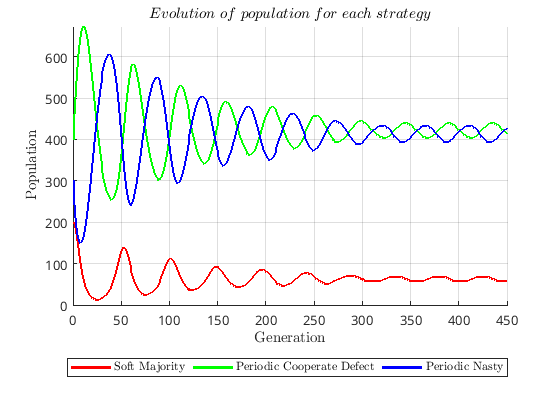
\includegraphics[width=0.8\textwidth]{media/increasing_oscillations_dec}
    \caption{Increasing oscillations Dec Plot}
\end{figure}

\subsection{Disordered oscillations}
When examining the disordered oscillations, the closest we could get was the "off" method. However the phenomenon ended quicker, at around 260 generations and the final state had soft majority and periodic ultra kind strategies go extinct. "dec" and "pop" had very similar behavior to the attenuated oscillatory movements meeting.
\begin{figure}[H]
    \centering
    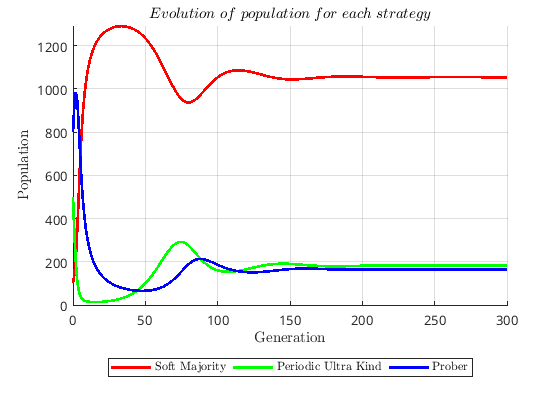
\includegraphics[width=0.8\textwidth]{media/disordered_oscillations_off.png}
    \caption{Disordered oscillations off Plot}
\end{figure}

\subsection{Population size sensitivity}
Going forward the paper decides to explore the tournament's sensitivity in slight changes of various parameters starting with the initial population size. Other than the fact that the crucial point where the oscillations stop gets shifted at periodic defect-defect-cooperate population: 235 into 236, instead of 244 into 245, the plots are the same. The rounding method used is "dec".

\begin{figure}[H]
    \centering
    \includegraphics[width=0.8\textwidth]{media/population_size_sensitivity_before_dec.png}
    \caption{Population size sensitivity before Dec Plot}
\end{figure}

\begin{figure}[H]
    \centering
    \includegraphics[width=0.8\textwidth]{media/population_size_sensitivity_after_dec.png}
    \caption{Population size sensitivity after Dec Plot}
\end{figure}

\subsection{Population size sensitivity 2}
The second population sensitivity experiment appears to have the same shift where this time, 159 into 160 becomes 181 into 182. The rounding method used is "pop".
\begin{figure}[H]
    \centering
    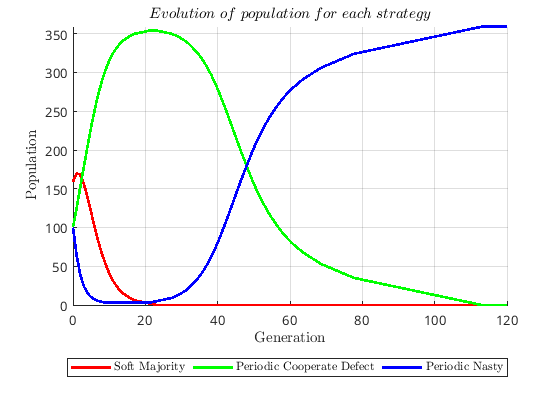
\includegraphics[width=0.8\textwidth]{media/population_size_sensitivity_2_before_pop.png}
    \caption{Population size sensitivity 2 before Pop Plot}
\end{figure}
\begin{figure}[H]
    \centering
    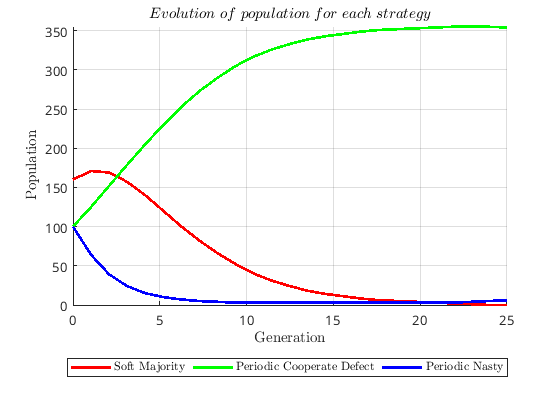
\includegraphics[width=0.8\textwidth]{media/population_size_sensitivity_2_after_pop.png}
    \caption{Population size sensitivity 2 after Pop Plot}
\end{figure}

\subsection{Game length sensitivity}
This experiment examines the case of changing the game's length or the number of rounds played by the players each generation. In the before state the reach higher peaks in the paper than our example, however we manage to capture the transition from periodic movements to attenuated oscillations. The rounding method used is "dec".
\begin{figure}[H]
    \centering
    \includegraphics[width=0.8\textwidth]{media/game_length_sensitivity_before_dec.png}
    \caption{Game length sensitivity before Dec Plot}
\end{figure}
\begin{figure}[H]
    \centering
    \includegraphics[width=0.8\textwidth]{media/game_length_sensitivity_after_dec.png}
    \caption{Game length sensitivity after Dec Plot}
\end{figure}

\subsection{Payoff matrix sensitivity}
This meeting highlights the effects a slight change to one of the payoff matrix values can have on the results. In the before state we see increasing oscillations and after changing the defector's exploiting payoff these oscillations become periodic. We perfectly replicate the paper's results using the "dec" method. 
\begin{figure}[H]
    \centering
    \includegraphics[width=0.8\textwidth]{media/payoff_matrix_sensitivity_before_dec.png}
    \caption{Payoff matrix sensitivity before Dec Plot}
\end{figure}
\begin{figure}[H]
    \centering
    \includegraphics[width=0.8\textwidth]{media/payoff_matrix_sensitivity_after_dec.png}
    \caption{Payoff matrix sensitivity after Dec Plot}
\end{figure}

\subsection{Rounding method sensitivity}
The final category of minor changes leading to different results is the rounding method. Though out the meetings analysis we have highlighted the importance of the rounding method since to replicate the paper's results we resorted to creating more than one methods, alternating between all of them to better illustrate the effects mentioned in the paper. On the first example we see periodic movements become attenuated oscillations and ultimately steady states. The rounding method used in the before state is "dec" and in the after state it is "off" or no rounding.
\begin{figure}[H]
    \centering
    \includegraphics[width=0.8\textwidth]{media/rounding_method_sensitivity_before_dec.png}
    \caption{Rounding method sensitivity before Plot}
\end{figure}
\begin{figure}[H]
    \centering
    \includegraphics[width=0.8\textwidth]{media/rounding_method_sensitivity_after_off.png}
    \caption{Rounding method sensitivity after Plot}
\end{figure}
The second example is best displayed using the "pop" method. Here we divide our initial populations with ten making rounding more important since we round an substantially larger section of the individual populations.
\begin{figure}[H]
    \centering
    \includegraphics[width=0.8\textwidth]{media/rounding_method_sensitivity_2_before_pop.png}
    \caption{Rounding method sensitivity 2 before Plot}
\end{figure}
\begin{figure}[H]
    \centering
    \includegraphics[width=0.8\textwidth]{media/rounding_method_sensitivity_2_after_pop.png}
    \caption{Rounding method sensitivity 2 after Plot}
\end{figure}
\setcounter{figure}{0}
\section{Imitation dynamics-Markov Theory}
\subsection{Imitation dynamics-brief review }
This second part of the project was implemented in a completely different way. Object-oriented programming was not the basis here. The logic is implementing 1 on 1 tournaments of 3 players, where populations change on the basis of implemented rules and states.
\\ \textbf{1)Here's how to run the Markov chain theoretical calculation of the one-step transition matrix:}
\\
 All the files required for the theoretical calculation of the one-step transition matrix are inside the \mintinline{matlab}{MarkovTheory} directory.
\
In function \mintinline{matlab}{initializeT.m}, we can choose the payoff matrix $(R, S, T, P)$, the total population \mintinline{matlab}{n}, the vector \mintinline{matlab}{chosen} of strategies to compete and \mintinline{matlab}{rounds}, the number of rounds per match (not important for the calculation purposes).
\
The script to run in order to obtain the theoretical one-step transition matrix is \mintinline{matlab}{MarkovTournament.m}.
\
At the end of the execution, all the plots are generated and a file named \mintinline{matlab}{TheoryOutput.mat} is created in the same directory, with the value of the one-step transition matrix, under the name \mintinline{matlab}{MTheory}.
\\
\textbf{2)How to run the simulated calculation of the one-step and the k-step (k big) transition matrix:}
\\
All the files required for the simulated calculation of the one-step and k-step (k big) transition matrices are inside the \mintinline{matlab}{MarkovSim} directory. Since for comparison reasons the result of the theoretical calculation, i.e. the matrix \mintinline{matlab}{MTheory}, is needed by the simulated calculation, the communication is achieved via \mintinline{matlab}{save/load} of this variable, through the constructed file \mintinline{matlab}{TheoryOutput.mat} inside the \mintinline{matlab}{MarkovTheory} directory and the variable is loaded automatically in the simulation’s workspace. In order that this communication can be achieved without any issues, the two directories \mintinline{matlab}{MarkovTheory} and \mintinline{matlab}{MarkovSim} should be saved in the same parent directory.
\
In function \mintinline{matlab}{initializeT.m}, one can choose the total population \mintinline{matlab}{N}, the \mintinline{matlab}{chosen} strategies to compete and the payoff matrix (they should all be the same with the ones of the theoretical calculation, for comparison purposes), as well as the \mintinline{matlab}{rounds} per match, the number of repetitions per initial state \mintinline{matlab}{numofreps} and the number of generations (meetings) per repetition, \mintinline{matlab}{ngens}. 
\
At the end of the execution, all the plots are generated and comparison results are reported. In order for the plots to draw properly, one should wait until the Matlab cursor reappears in the Command Window. 
\
In both initialization functions, if one wishes to add a new strategy, it is required to add a new id number for it, its name, its strategy vector and the possibility for a player of this strategy to choose C as his first move in the appropriate maps therein.

\subsection{Computation of Expected Average Payoff using Markov Chains}
In one round of the game, the outcome can be CC, CD, DC, or DD, where C = cooperation and D = defection. In each pair, the first letter represents the choice of the first player and the second the choice of the second player. In games where both players adopt strategies based on memory of the previous round (memory-one strategies), or generally in case of finite-memory strategies, the game can be modeled as a finite-state Markov chain, where the system transitions between the four states CC, CD, DC, DD. The conditional probabilities of any future event depend only on the current state and are independent of any past event.

Thus, the one-step transition matrix \( M \) has the form:

\[
M =
\begin{bmatrix}
p(\text{CC}|\text{CC}) & p(\text{CC}|\text{CD}) & p(\text{CC}|\text{DC}) & p(\text{CC}|\text{DD}) \\
p(\text{CD}|\text{CC}) & p(\text{CD}|\text{CD}) & p(\text{CD}|\text{DC}) & p(\text{CD}|\text{DD}) \\
p(\text{DC}|\text{CC}) & p(\text{DC}|\text{CD}) & p(\text{DC}|\text{DC}) & p(\text{DC}|\text{DD}) \\
p(\text{DD}|\text{CC}) & p(\text{DD}|\text{CD}) & p(\text{DD}|\text{DC}) & p(\text{DD}|\text{DD})
\end{bmatrix}
\]




For example, \( p(\text{CD}|\text{DC}) = p(X_{k+1} = \text{CD} | X_k = \text{DC}) \) is the probability that the next state is CD, given the current state is DC (the first player chooses C and the second D, while their previous moves were D and C, respectively).

Assuming independence of the players' choices:
\[
p(\text{CD}|\text{DC}) = p_X(C|\text{DC}) \cdot p_Y(D|\text{DC}) = p_X(C|\text{DC}) \cdot (1 - p_Y(C|\text{DC}))
\]
where \[
 p_X(C|\text{DC}) 
\]
is the probability that the first player chooses C for his next move, when the previous state was DC, and 
\[
 p_Y(D|\text{DC}) 
\]
is the probability that the second player chooses D for his next move, when the previous state was DC. It is important to be able to calculate  the conditional probabilities: \[
p_X(C|\text{CC}) ,p_X(C|\text{CD}), p_X(C|\text{DC}), p_X(C|\text{DD}) 
\]
that is, the probabilities for a player to choose C given that the previous state was CC, or CD, or DC, or DD, which are dependent on the specific strategy that the player has adopted.

Let us define:

\[
\mathbf{p} = (p_1, p_2, p_3, p_4) = (p_X(C|\text{CC}), p_X(C|\text{CD}), p_X(C|\text{DC}), p_X(C|\text{DD}))
\]
\[
\mathbf{q} = (q_1, q_2, q_3, q_4) = (p_Y(C|\text{CC}), p_Y(C|\text{CD}), p_Y(C|\text{DC}), p_Y(C|\text{DD}))
\]
the strategy vectors for the first player, and the second player, respectively. Vector $\mathbf{p}$ can be calculated for each strategy.
For example:
\begin{itemize}
  \item Random strategy: \( \mathbf{p} = (0.5, 0.5, 0.5, 0.5) \)
  \item All-C: \( \mathbf{p} = (1, 1, 1, 1) \)
  \item All-D: \( \mathbf{p} = (0, 0, 0, 0) \)
  \item Tit-For-Tat: \( \mathbf{p} = (1, 0, 1, 0) \)
  \item Generous Tit-For-Tat (GTFT): \( \mathbf{p} = (1, q, 1, q) \), since, in comparison with Tit-for-Tat, when the opponent has played D, GTFT responds with D with a probability of $1-q$
  \item Pavlov (Win State Lose Shift): \( \mathbf{p} = (1, 0, 0, 1) \)
\end{itemize}

Using these vectors, the one-step transition matrix \( M \) becomes:

\[
M =
\begin{bmatrix}
p_1 q_1 & p_1 (1 - q_1) & (1 - p_1) q_1 & (1 - p_1)(1 - q_1) \\
p_2 q_3 & p_2 (1 - q_3) & (1 - p_2) q_3 & (1 - p_2)(1 - q_3) \\
p_3 q_2 & p_3 (1 - q_2) & (1 - p_3) q_2 & (1 - p_3)(1 - q_2) \\
p_4 q_4 & p_4 (1 - q_4) & (1 - p_4) q_4 & (1 - p_4)(1 - q_4)
\end{bmatrix}
\]
Each row of \( M \) must sum to 1. Let it be noted that in the second row, the system transits to a CD state (given the current state CC, CD, DC, DD) and thus the second player transits to a D state. For that reason, \(
q_3 = p_Y(C|\text{DC}) 
\), which represents the probability that the second player chooses C, given the previous state DC and not  \(
q_2 
\)  is used. Similar observations can be made about the third row.
It is also important to be able to calculate the unconditional (marginal) probabilities that the system will be driven in a CC, CD, DC or DD state, and how these are evolving through generations. 
Let \( v_k \) be the vector of unconditional probabilities at step \( k \):
\[
v_k = \begin{bmatrix}
p(X_k = \text{CC}) ,  p(X_k = \text{CD}) ,  p(X_k = \text{DC}) ,  p(X_k = \text{DD})
\end{bmatrix}
\]

Then, using the law of total probability: \[
\begin{aligned}
p(X_{k+1} = CD) &= p(X_{k+1} = CD \mid X_k = CC) \, p(X_k = CC) \\
&\quad + p(X_{k+1} = CD \mid X_k = CD) \, p(X_k = CD) \\
&\quad + p(X_{k+1} = CD \mid X_k = DC) \, p(X_k = DC) \\
&\quad + p(X_{k+1} = CD \mid X_k = DD) \, p(X_k = DD) \\
&= 
\begin{bmatrix}
p(CD \mid CC) , p(CD \mid CD) , p(CD \mid DC) , p(CD \mid DD)
\end{bmatrix}
\cdot
\begin{bmatrix}
p(X_k = CC) \\
p(X_k = CD) \\
p(X_k = DC) \\
p(X_k = DD)
\end{bmatrix}
\end{aligned}
\]

In the last equation, we used the simpler notation adopted in the transition matrix \( M \). That is, \( p(X_{k+1} = CD) \), which is an element of the vector \( v_{k+1} \), equals the inner product of the second row of the one-step transition matrix \( M \) and the vector \( v_k \). Therefore, overall, the temporal evolution of \( v_k \) follows \( v_{k+1} = M v_k \), and recursively \( v_{k+1} = M^{k+1} v_0 \), where \( v_0 \) is the vector of unconditioned probabilities for the system to be in one of the states \( CC, CD, DC, DD \) at the step when the players make their initial moves.  Thus, matrix \( M^m \) is the matrix of conditional probabilities over \( m \) steps (the \( m \)-step transition matrix), and includes all the conditional probabilities for transitioning from any current state \( CC, CD, DC, DD \) to any other state \( CC, CD, DC, DD \) in \( m \) steps of the game (Chapman-Kolmogorov equations).


It is proven that when the Markov chain is irreducible and ergodic, the vector \( v_k \) of unconditioned probabilities converges \( (\lim_{k \to \infty} v_k = \pi) \) to the stationary distribution \( \pi \), which is also given by the convergent limit 

\[
\pi = \lim_{n \to \infty} \frac{1}{n} \sum_{k=0}^{n-1} v_0 M^k
\]

When this limit exists, it is independent of \( v_0 \). Clearly, for \( \pi \), it holds that \( \pi M = \pi \) (from the relation \( v_{k+1} = M v_k \) in the limit \( k \to \infty \)), and the sum of the elements of \( \pi \) is equal to 1, as it represents the unconditioned probabilities, in the steady state, that the system is found in one of the states \( CC, CD, DC, DD \). 

Then, the elements of each column of the matrix \( M^m \), for large \( m \), approach the same value, since the conditional probability of transitioning to a state in \( m \) steps becomes independent of the current state of the system. Knowing, for a game between two opponents \( X \) and \( Y \), the vector \( \pi \) with the long-term probabilities of the system being in any of the states \( CC, CD, DC, DD \), it is clear that we can calculate the average expected pay-off per round for each of the two opponents, using the formulas:

\[
s_X = \pi S_X = \pi
\begin{bmatrix}
R \\
S \\
T \\
P
\end{bmatrix}
\quad \text{and} \quad
s_Y = \pi S_Y = \pi
\begin{bmatrix}
R \\
T \\
S \\
P
\end{bmatrix}
\]

respectively.
\section{Theoretical calculation of the state transition matrix using Markov chains}
In the sequel, we will consider a tournament between $M=3$ strategies with an imitating behavior, let us call them $A, \ \ B$ and $C$, with $n_1,\ \ n_2$ and $n_3$ being their respective population at a certain generation. During all generations, the total population remains constant at $N=n_1+n_2+n_3$. At each generation, we consider a two-by-two round robin tournament between all the players, where each player of strategy $X$ plays a number of games with opponents $Y$ of his strategy group, or with opponents from the other strategies, according to the table given here after:
\\\\
\begin{center}
    

\begin{tabular}{|c|c|c|c|}
 \hline
 \backslashbox{$X$}{$Y$} & $A$ & $B$ & $C$ \\ 
 \hline
$A$ & $\frac{n_1(n_1-1)}{2}$ & $n_1n_2$ & $n_1n_3$ \\
 \hline
$B$ &  & $\frac{n_2(n_2-1)}{2}$ & $n_2n_3$ \\
 \hline
$C$ &  &  & $\frac{n_3(n_3-1)}{2}$ \\
 \hline
\end{tabular}

\end{center}

From our previous analysis, considering the Markov chain of a certain game between two players, having as states all the possible outcomes of the game $(CC, \ \ CD, \ \ DC, \ \ DD)$, we were able to calculate the mean expected payoff for each one of the two players. More precisely, having the strategy vectors $$\mathbf{p}=(p_X(C|CC)\ \ p_X(C|CD)\ \ p_X(C|DC)\ \ p_X(C|DD))$$ and $$\mathbf{q}=(p_Y(C|CC)\ \ p_Y(C|CD)\ \ p_Y(C|DC)\ \ p_Y(C|DD))$$ we can calculate the one-step transition matrix $M(\mathbf{p}, \mathbf{q})$, then the stationary distribution $\pi$ from $\pi M=\pi$ and $\sum_{i}\pi(i)=1$ and finally the mean expected payoff of each one of the two players as 
$$s_X=\pi S_X=\pi
\begin{bmatrix}
R \\
S \\
T \\
P 
\end{bmatrix}\ ,
s_Y=\pi S_Y=\pi
 \begin{bmatrix}
R \\
T \\
S \\
P 
\end{bmatrix}$$

with

\begin{center}
 \begin{tabular}{|c|c|c|c|}
\hline
 & $C$ & $D$ \\
 \hline
$C$ & \shortstack{$R$ \\ $R$} & \shortstack{$T$ \\ $S$} \\
\hline
$D$ &  \shortstack{$S$ \\ $T$}  &  \shortstack{$P$ \\ $P$}  \\
\hline
\end{tabular} 
\end{center}
the game payoff matrix.
In a meeting (tournament) of 3 strategies, let us denote with
$$\mathbf{P}=[P_{AA}^A,\ \ P_{BB}^B,\ \ P_{CC}^C,\ \ P_{AB}^A,\ \ P_{AB}^B,\ \ P_{AC}^A,\ \ P_{AC}^C,\ \ P_{BC}^B,\ \ P_{BC}^C]$$
a vector comprising all the payoffs between two players. In $\mathbf{P}$, $P_{XY}^X$ denotes the payoff for player $X$ in a match between $X$ and $Y$ and $P_{XY}^Y$ the payoff of player $Y$ in the same match. Obviously, considering all the matches in a meeting, if each match comprises $U$ rounds, the total mean expected payoff for each one of the three strategies is given by
$$\text{strategy A:} \ \ SC_A=[n_1(n_1-1)P_{AA}^A+n_1n_2P_{AB}^A+n_1n_3P_{AC}^A]U$$

$$\text{strategy B:} \ \ SC_B=[n_1n_2P_{AB}^B+n_2(n_2-1)P_{BB}^B+n_2n_3P_{BC}^B]U$$

$$\text{strategy C:} \ \ SC_C=[n_1n_3P_{AC}^C+n_2n_3P_{BC}^C+n_3(n_3-1)P_{CC}^C]U$$
Note here that in a match between two players of the same strategy, the strategy payoff is $2P_{XX}^X$. We are now ready, for the specific choice of strategies $A, B$ and $C$ and for all combinations of populations $n_1, \ \ n_2, \ \ n_3$, such that $n_1+n_2+n_3=N$, $n_i\in \mathbb{Z}$, $0\le n_i\le N$, to calculate the mean expected total payoffs for the three strategies $(SC_A,\ \  SC_B ,\ \ SC_C)$ and find which can be the next state. In general, being at a certain state $(n_1, \ \ n_2, \ \ n_3)$, the next state can be one of the following: $(n_1, \ \ n_2, \ \ n_3)$, or $(n_1+1, \ \ n_2-1, \ \ n_3)$, or $(n_1+1, \ \ n_2, \ \ n_3-1)$, or $(n_1-1, \ \ n_2+1, \ \ n_3)$, or $(n_1, \ \ n_2+1, \ \ n_3-1)$, or $(n_1-1, \ \ n_2, \ \ n_3+1)$, or $(n_1, \ \ n_2-1, \ \ n_3+1)$, as far as $n_1\pm1, \ \ n_2\pm1, \ \ n_3\pm1$ remain integers in the region $[0,N]$.
\\\\
After ordering the three strategies in descending order, based on their scores ${SC}_A$, ${SC}_B$, ${SC}_C$ in a meeting, and supposing that the strategies have $n_1$, $n_2$, $n_3$ players respectively in the current state, we have the following mutually independent cases for the movements of a player from a state to another one, together with their respective probabilities.


\begin{center}
    

\begin{tabular}{|c|c|c|c|}
 \hline
 Relations between \\scores and populations & Current state & Next state & Probability \\ 
 \hline
Rule00: $SC_A$, $SC_B=$ $SC_C=0$ & $(n_1,\ \ 0,\ \ 0)$ & $(n_1,\ \ 0,\ \ 0)$ & $1$ \\
 \hline
Rule01: $SC_A>$ $SC_B,$ $SC_C=0$ & $(n_1,\ \ n_2,\ \ 0)$ & $(n_1+1,\ \ n_2-1,\ \ 0)$ & $\frac{n_2}{n_1+n_2}$ \\
 
 &  & $(n_1,\ \ n_2,\ \ n_3)$ & $\frac{n_1}{n_1+n_2}$ \\
 \hline
Rule02: $SC_A=$ $SC_B,$ $SC_C=0$ & $(n_1,\ \ n_2,\ \ 0)$ & $(n_1,\ \ n_2,\ \ 0)$ & $\frac{1}{2}$ \\
 
 &  & $(n_1+1,\ \ n_2-1,\ \ 0)$ & $\frac{1}{2}\frac{n_2}{n_1+n_2}$ \\
 
 &  & $(n_1-1,\ \ n_2+1,\ \ 0)$ & $\frac{1}{2}\frac{n_1}{n_1+n_2}$ \\
 \hline
Rule03: $SC_A>$ $SC_B>$ $SC_C$ & $(n_1,\ \ n_2,\ \ n_3)$ & $(n_1,\ \ n_2,\ \ n_3)$ & $\frac{n_1}{n_1+n_2+n_3}$ \\

 &  & $(n_1+1,\ \ n_2-1,\ \ n_3)$ & $\frac{n_2}{n_1+n_2+n_3}$ \\

 &  & $(n_1+1,\ \ n_2,\ \ n_3-1)$ & $\frac{n_3}{n_1+n_2+n_3}$ \\
 \hline
Rule04: $SC_A=$ $SC_B>$ $SC_C$ & $(n_1,\ \ n_2,\ \ n_3)$ & $(n_1,\ \ n_2,\ \ n_3)$ & $\frac{1}{2}\frac{n_1+n_2}{n_1+n_2+n_3}$ \\

 &  & $(n_1+1,\ \ n_2-1,\ \ n_3)$ & $\frac{1}{2}\frac{n_2}{n_1+n_2+n_3}$ \\

 &  & $(n_1-1,\ \ n_2+1,\ \ n_3)$ & $\frac{1}{2}\frac{n_1}{n_1+n_2+n_3}$ \\

 &  & $(n_1+1,\ \ n_2,\ \ n_3-1)$ & $\frac{1}{2}\frac{n_3}{n_1+n_2+n_3}$ \\

 &  & $(n_1,\ \ n_2+1,\ \ n_3-1)$ & $\frac{1}{2}\frac{n_3}{n_1+n_2+n_3}$ \\
 \hline
Rule05: $SC_A>$ $SC_B=$ $SC_C$ \\ (can be incorporated in rule 03) & $(n_1,\ \ n_2,\ \ n_3)$ & $(n_1,\ \ n_2,\ \ n_3)$ & $\frac{n_1}{n_1+n_2+n_3}$ \\

 &  & $(n_1+1,\ \ n_2-1,\ \ n_3)$ & $\frac{n_2}{n_1+n_2+n_3}$ \\

 &  & $(n_1+1,\ \ n_2,\ \ n_3-1)$ & $\frac{n_3}{n_1+n_2+n_3}$ \\
 \hline
Rule06: $SC_A=$ $SC_B=$ $SC_C$ & $(n_1,\ \ n_2,\ \ n_3)$ & $(n_1,\ \ n_2,\ \ n_3)$ & $\frac{1}{3}$ \\

 &  & $(n_1+1,\ \ n_2-1,\ \ n_3)$ & $\frac{1}{3}\frac{n_2}{n_1+n_2+n_3}$ \\

 &  & $(n_1+1,\ \ n_2,\ \ n_3-1)$ & $\frac{1}{3}\frac{n_3}{n_1+n_2+n_3}$ \\

 &  & $(n_1-1,\ \ n_2+1,\ \ n_3)$ & $\frac{1}{3}\frac{n_1}{n_1+n_2+n_3}$ \\

 &  & $(n_1,\ \ n_2+1,\ \ n_3-1)$ & $\frac{1}{3}\frac{n_3}{n_1+n_2+n_3}$ \\

 &  & $(n_1-1,\ \ n_2,\ \ n_3+1)$ & $\frac{1}{3}\frac{n_1}{n_1+n_2+n_3}$ \\

 &  & $(n_1,\ \ n_2-1,\ \ n_3+1)$ & $\frac{1}{3}\frac{n_2}{n_1+n_2+n_3}$ \\

 \hline

\end{tabular}
\end{center}

In the table above, we have supposed that a player is chosen randomly from the strategies which have non zero populations in the meeting and chooses randomly, with equal probability, to move to one of the strategies that scored the most in the meeting (more than one, if they draw).
\\
For example, in the case $SC_A=SC_B=SC_C$ we can remain in the same state $(n_1,\ \ n_2,\ \ n_3)$ if, either a player is chosen randomly from strategy $A$ with probability $\frac{n_1}{n_1+n_2+n_3}$ and moves to the same strategy with probability $\frac{1}{3}$, or a player is chosen from strategy $B$ and remains to $B$ with probability $\frac{1}{3}\frac{n_2}{_1+n_2+n_3}$, or a player is chosen from strategy $C$ and remains to $C$ with probability $\frac{1}{3}\frac{n_3}{n_1+n_2+n_3}$, all the probabilities summing to $\frac{1}{3}$. In an analogous manner, we have calculated all the reported state transitions in the table.
\\\\
We can follow the above described state transition rules, for each combination of possible strategy populations (integers $n_1, \ \ n_2, \ \ n_3$ such that $\sum_{i}n_i=N, n_i\in \mathbb{Z},\ \ n_i\in [0,N]$). We can provide all possible combinations by changing $n_1$ from $0$ to $N$, then for each $n_1$ changing $n_2$ from $0$ to $N-n_1$ and obtaining for each combination of $n_1, \ \ n_2$ the respective $n_3$ from $n_3=N-n_1-n_2$. There is a total of $(N+1)+N+(N-1)+...+2+1=\frac{((N+1)+1)(N+1)}{2}=\frac{(N+1)(N+2)}{2}$ combinations.
\\\\
Concerning now our MATLAB realization, in the \mintinline{matlab}{initialize()} function, we choose the total population, the payoff matrix, the number of rounds, and the three strategies to compete with their respective strategy vectors $\mathbf{p}$. The main script, \mintinline{matlab}{MarkovTournament.m}, calls \mintinline{matlab}{initialize()}, then calls the function \mintinline{matlab}{tournamentpayoffs} which returns the mean expected payoff for each of the player couples in a certain match (A vs A, B vs B, C vs C, A vs B, A vs C, B vs C). In order to calculate the payoffs, \mintinline{matlab}{tournamentpayoffs} calls function \mintinline{matlab}{payoff()}.
\begin{lstlisting}[caption=Function payoff]
    function [M, pi, payoff1, payoff2] = payoff(p, q, R, S, T, P)
    
    % Calculate transition matrix 
    M = transitionMatrix(p, q);

    % Solve symbolically the equations πM=π, Σπi=1, when π=[x y z t]
    % Symbolic variables
    syms x y z t;
    % Solution
    [solx, soly, solz, solt] = solve([x y z t]*M(:,1) == x, [x y z t]*M(:,2) == y,...
                                     [x y z t]*M(:,3) == z, [x y z t]*M(:,4) == t,...
                                      x + y + z + t == 1, [x y z t]);
    
    % Stationary distribution π
    pi = [solx, soly, solz, solt];

    % Long-run average expected pay-offs of the two players
    payoff1 = double(pi*[R;S;T;P]);
    payoff2 = double(pi*[R;T;S;P]);


end
\end{lstlisting}
This function calculates the transition matrix M by calling the function \mintinline{matlab}{transitionMatrix()}, resolves the equations $\pi M=\pi$, $\sum_{i}\pi(i)=1$ in order to obtain the stationary distribution vector $\pi$ and then finds the mean expected payoffs $P_{XY}^X$ and $P_{XY}^Y$.
\\\\
Then, in a double loop, all triplets ($n_1, \ \ n_2, \ \ n_3$) are created, and for each one of them, all the above mentioned rules are examined to find the one which is satisfied, which will provide the next states to which the transition can be done, together with the respective probability for each one of them.
\\\\
The current states are stored in the matrix \mintinline{matlab}{allcurrentstates}, their respective next states in the matrix \mintinline{matlab}{allnextstates}, and the respective probabilities in the matrix \mintinline{matlab}{allprobs}. Because from one current state we can transit to more than one next states, the elements of \mintinline{matlab}{allcurrentstates} are non unique.
\\\\
We find all the unique elements of \mintinline{matlab}{allcurrentstates}, in the matrix \mintinline{matlab}{allcurrentuniquestates}, which subsequently also comprises the unique names of all the states. We can then build the one-step transition matrix by finding to which index of the matrix \mintinline{matlab}{allcurrentuniquestates}, corresponds the current state \mintinline{matlab}{allcurrentstates(i)} and its respective next state, \\\mintinline{matlab}{allnextstates(i)}. By using MATLAB's \mintinline{matlab}{dtmc}, we construct a Markov chain model and plot the heatmaps of the one-step transition matrix, the k-step transition matrix $M^k$ for a certain big $k$ (for example $k=100$) and a movie of how the heatmap of $M^k$ changes as $k$ changes from $0$ to $k$ and finally a state transition diagram.
\\\\ 
For the three strategy tournaments, we can choose between the well known strategies All-C, All-D, Random, Pavlov, Tit-for-Tat and Generous Tit-for-Tat. For these strategies we can easily calculate their strategy vector $\mathbf{p}$. Moreover, we can choose between some strategies which are called zero determinant strategies.
\\\\
A player using such a strategy, can enforce a linear relation $\alpha s_X+\beta s_Y+\gamma=0$, or $(s_X-P)=\chi(s_Y-P), \ \ \chi\ge 1$ between the scores $s_X$ and $s_Y$. These strategies are based on the fact that it can be proven that, the inner product of a game's stationary distribution $\pi$ and an arbitrary $4\times 1$ vector $\mathbf{f}=[f_1,\ \ f_2,\ \ f_3,\ \ f_4]^T$ equals the determinant of a matrix:
\\\\
$\pi \cdot \mathbf{f}=\det\Big($
$
 \begin{bmatrix}
-1+p_1q_1 & -1+p_1 & -1+q_1 & f_1 \\
p_2q_3 & -1+p_2 & q_3 & f_2 \\
p_3q_2 & p_3 & -1+q_2 & f_3 \\
p_4q_4 & p_4 & q_4 & f_4 
\end{bmatrix} 
\Big)
$
$=\det[\overline{\mathbf{r}}(\mathbf{p},\mathbf{q})\ \ \tilde{\mathbf{p}}(\mathbf{p})\ \ \tilde{\mathbf{q}}(\mathbf{q})\ \ \mathbf{f}]$ with $\mathbf{p}=(p_1,\ \ p_2,\ \ p_3,\ \ p_4)$ and $\mathbf{q}=(q_1,\ \ q_2,\ \ q_3,\ \ q_4)$ the two strategy vectors.
\\\\
Notice here that the second column $\tilde{\mathbf{p}}$ of the matrix is solely under the control of $X$ while the third column $\tilde{\mathbf{q}}$ is solely under the control of $Y$, because they depend on $\mathbf{p}$ and $\mathbf{q}$, respectively, which $X$ and $Y$, respectively, can choose at their will. Player $X$ can choose $\mathbf{p}$ such that $\tilde{\mathbf{\mathbf{p}}}$ becomes equal to $\mathbf{f}$, subsequently zeroing the determinant and obtaining $\pi\cdot \mathbf{f}=0$ (hence the name zero determinant). By choosing $\mathbf{f}=\alpha S_X+\beta S_Y+\gamma\mathbf{1}$ with $\mathbf{1}=[1\ \ 1\ \ 1\ \ 1]^T$, it can be proven that $\alpha s_X+\beta s_Y+\gamma=0$, while by choosing $\mathbf{f}=(S_X-P\mathbf{1})-\chi(S_Y-P\mathbf{1})$ it can be proven that $(s_X-P)=\chi(s_Y-P)$.
\\\\
In the case $\alpha s_X+\beta s_Y+\gamma=0$, one could suppose that $X$ could
choose $\beta=0$ and impose his score $s_X$, but this is proven to be non feasible. On the contrary, it is absolutely feasible for $X$ to choose $\mathbf{p}$ such that $\tilde{\mathbf{p}}=\mathbf{f}=\alpha S_X+\beta S_Y+\gamma \mathbf{1}$ and thus $\pi \cdot \mathbf{f}=0$ and with the choice $\alpha=0$, impose the score of $Y$ to $s_Y-\frac{\gamma}{\beta}$, and this can be done independently of Y's strategy. In the same way, it is feasible for $Y$ to choose $\mathbf{q}$ such that $\tilde{\mathbf{q}}=\mathbf{f}=\alpha S_X+\beta S_Y+\gamma\mathbf{1}$ and thus $\pi \cdot \mathbf{f}=0$ and with the choice $\beta=0$ impose the score of his opponent $X$ to $s_X=-\frac{\gamma}{\alpha}$, independently of X's strategy.
\\\\
We use for example the strategies SET-2 which forces the opponent's payoff to be 2 regardless of what strategy the opponent uses, and SET-3. For SET-2, \\ $\mathbf{p}=(p_X(C|CC)\ \ p_X(C|CD)\ \ p_X(C|DC)\ \ p_X(C|DD))=(0.75\ \ 0.25\ \ 0.5\ \ 0.25)$ and for SET-3 $\mathbf{p}=(1\ \ 0.9\ \ 0.15 \ \ 0.1)$. We also use the generous zero determinant strategy GEN-2 with $\mathbf{p}=(1\ \ 0.5625\ \ 0.5\ \ 0.125)$.
\\\\
Similarly, $X$ can choose $\mathbf{p}$ such that $\tilde{\mathbf{p}}=\phi \mathbf{f}=\phi[(S_X-P\mathbf{1})-\chi(S_Y-P\mathbf{1})],\ \ \chi\ge1,\ \ 0< \phi\le \frac{P-S}{(P-S)+\chi(T-P)}$ and thus obtain $\pi \cdot \mathbf{f}=0$ and impose an extortionate share of payoffs $(s_X-P)=\chi(s_Y-P)$. We have used the extortionate strategies EXT-2 with $\chi=2$ and $\mathbf{p}=(0.875\ \ 0.4375\ \ 0.375 \ \ 0)$ and EXT-5 with $\chi=5$ and $\mathbf{p}=[0.68 \ \ 0.16\ \ 0.36\ \ 0]$. We note here that Tit-for-Tat results as an extortionate zero determinant strategy with the strategy vector $(1\ \ 0\ \ 1\ \ 0)$, in the special case $\chi=1$ and $\phi=\frac{1}{5}$, thus imposing $s_X=s_Y$, implying fairness.
\\\\
We report the simulation results in the case of a tournament comprising the three strategies. GEN-2, SET-3 and Tit-for-Tat. With $N=9$ being the total population, there are 55 different states. We give hereafter the heatmaps of $M,\ \ M^8$ and $M^{100}$ (Figures 1,2 pages 38).
\\\\
For the k-step transition matrix $M^k$, for $k$ big, we see that all states end up to either state $1$ (state$(0,\ \ 0,\ \ 9)$) or state $10$ (state$(0,\ \ 9,\ \ 0)$) or state $55$ (state$(9,\ \ 0,\ \ 0)$), which are the equilibrium states. In these cases, the winner is Tit-for-Tat, or SET-3, or GEN-2, respectively(Figure 3, page 39). We finally give a digraph of the Markov chain(Figure 4, page 40).

\section{Simulation calculated state transition matrices}


We simulated in MATLAB the evolutionary imitation dynamics. In order to be able to also simulate zero determinant strategies, at the lowest level, in function \mintinline{matlab}{randomplay()}, for each strategy in a game described by its strategy vector $\mathbf{p}$, we construct a $4\times rounds$ matrix, where each row is a random vector of 'round' elements, '0's for 'C' and '1's for 'D', where 'C' is present in each vector with a probability $p(C|CC),\ \ p(C|CD),\ \ p(C|DC)$ and $p(C|DD)$, respectively. There are 'rounds' rounds in a match between two players. During a match between two players, depending on the outcome of the system's previous state $(CC,\ \ CD,\ \ DC,$ or $DD)$ a player can choose his response in the current round, by using an element  of the appropriate row of this premade matrix. We can guarantee (up to rounding errors) that the desired probabilities are exact when considering all the elements of the row and approximately exact when less elements of the row are used in a match. By simulation, we have seen that this strategy with the premade choices works slightly better than using a random generator each time at the level of a round in a match, in order to produce 'C' or 'D' with a specified probability. MATLAB's function \mintinline{matlab}{randperm()} for random permutations of integers was used to create the premade choice matrices. For deterministic strategies like All-C, All-D, Pavlov, Tit-for-Tat which have only '0's or '1's in their strategy vectors $\mathbf{p}$, the results obtained are exact (up to rounding errors).
\\\\
The function \mintinline{matlab}{playmatch()} is used to simulate a match of 'rounds' rounds between two players, following strategies with vectors $\mathbf{p}$ and $\mathbf{q}$, respectively, and with their respective premade choice matrices. For zero determinant strategies, the first move of the player is randomly chosen between 'C' or 'D' with probability 0.5 for each. This function also calculates the score of each player in a match, based on the game playoff matrix. The premade choice matrices are randomly recalculated for each match between two players.
\\\\
The function \mintinline{matlab}{gentournament()} realizes  a meeting between three strategies (a generation in evolutionary terms), where all matches between all possible pairs of players are played. For the number of matches between players belonging to two strategies, see the matrix in the beginning of the previous section. By summing, it can be easily seen that there are $\frac{N(N-1)}{2}$ matches in a meeting, N being the total constant population. After a match is finished, the total score of each strategy is updated according to the outcome of the match, also in function \mintinline{matlab}{gentournament()}. Finally, the same function, given the current state and the meeting scores for each one of the three strategies, calls the function \mintinline{matlab}{nxt()}, which calculates the next state of the system. After a meeting, one player is chosen randomly from the strategies with a non zero number of players and chooses, by imitation, to follow one of the strategies that scored the most in the meeting. The details of changing strategy for one player after a meeting, were described in the previous section and are realized in \mintinline{matlab}{nxt()}. Either a player moves from a strategy to another one (realized by the function \mintinline{matlab}{transferfromXtoY()} in \mintinline{matlab}{nxt()}), or we remain in the same state (realized by \mintinline{matlab}{remaintosamestate()}).
\begin{lstlisting}[caption= Abstract example from nxt.m: Three strategies with non-zero populations and the same pay-offs]
    
    if sortedS(1) > sortedS(2) && sortedS(2) > sortedS(3)
        fprintf('Rule 04: Three strategies with non zero populations and different pay-offs\n');
        fprintf('SA=%.2f, SB=%.2f, SC=%.2f \n',SA, SB, SC);
        % Transfer one player from the third to the first strategy
        nextstate = transferfromXtoY(3, 1, n, idx);

\end{lstlisting}
In both these functions, when a transition from the current state to a next state is realized, we add one to the one-step transition matrix, in each appropriate (row, column) element (depending on the transition). The rows of the matrix are at the end normalized to probabilities to transit, starting from one state, to other states, in the script \mintinline{matlab}{Markovsim.m}. The matrix is declared as \mintinline{matlab}{global Msim}.
\\\\
The evolution from one generation to the next is realized in \mintinline{matlab}{mutligen()}, which calls \mintinline{matlab}{gentournament()}, \mintinline{matlab}{ngens} times in order to obtain the final equilibrium states, useful for the calculation of the k-step (k big) transition matrix \mintinline{matlab}{Mk}.
\\\\
In the script \mintinline{matlab}{Markovsim.m}, in a double \mintinline{matlab}{for} loop, we create all the possible states, given a population of $N$ players ($\frac{(N+1)(N+2)}{2}$ states) and call \mintinline{matlab}{multimultigen()} to create the k-step transition matrix. \mintinline{matlab}{Markovsim.m} calls \mintinline{matlab}{initialize()}, where we can set the total population, the payoff matrix, the number of rounds in a match, the number of generations, the number of simulation runs starting from the same state and finally choose the three strategies to compete together with their strategy vectors and initial movements. After the end of the simulation, in \mintinline{matlab}{Markovsim.m}, by using MATLAB's \mintinline{matlab}{dtcm()} we create Markov chain models for the one-step and k-step transition matrices and plot their digraph with \mintinline{matlab}{graphplot()}. We also create heatmaps for the simulated transition matrices \mintinline{matlab}{Msim}, \mintinline{matlab}{Mk} and for their differences, $|Msim-M_{Theory}|, |Mk-{(M_{Theory})}^{ngens}|$ from their respective theoretically calculated ones, $M_{Theory}$ and ${(M_{Theory})}^{ngens}$. We used as a metric of the difference between the two matrices, the sum of all the absolute values of the differences between all their respective elements.
\\\\
The simulations are quite time consuming, as indicated from the table hereafter. The total population chosen was $N=9$ players.

\begin{center}
\begin{tabular}{|c|c|c|c|c|}
 \hline
 Rounds per match & Generations & Repetitions per state & Simulation time & Metric \\ 
 \hline
50 & 40 & 3 & 15 min & 16 \\
 \hline
100 &   45 & 10 & 1 hrs 50 min & 7.5 \\
 \hline
500 & 50 & 15 & 15 hrs & 7.14 \\
 \hline
\end{tabular}
\end{center}

Since in the case $N=9$ there are 36 matches per meeting (generation), this gives an average of 4.1 msec per round of execution time in the computer used. A simulation with 1000 rounds/match 50 generations and 100 repetitions per state would need almost 210 hours ($\textasciitilde 9$ days) of simulation time.
\\\\
For the last case in the table above, we report the heatmap of the simulated (\mintinline{matlab}{Msim}-Figure 5,page 41) and theoretical (\mintinline{matlab}{MTheory}-Figure 6,page 41) one-step transition matrices and of the absolute value of their difference in Figure 7, page 42, which appears to be minimal. The same holds for the heatmaps of the simulated k-step (k big) transition matrix (Figure 8, page 42), the respective theoretical one $(MTheory)^{ngen}$ (Figure 9, page 43) and the absolute value of their difference (Figure 10, page 43). In Figure 13,page 46, we report the values of the metric per row of the matrices, for the one-step (blue color) and the k-step (red color) transition matrix.
\\\\
In Figures 11 and 12, pages 44-45 we give the digraphs for the simulated one-step and k-step transition matrices, respectively. For comparison purposes the digraph for the respective theoretically computed one-step Matrix is given in Figure 14  (page 47) also. The three strategies competing were GEN-2, SET-3 and Tit-for-Tat. In Figures 15 and 16 (pages 48,49) we give the digraphs for the one-step and k-step matrices. In this case the strategies are All-C, All-D and Tit-for-Tat, using 50 rounds per match, 3 repetitions and 50 generations.


\newpage
\section{Heatmaps-State graphs}

\begin{figure}[h!]
    \centering
    \includegraphics[width=0.6\textwidth]{media/A.jpg}
    \caption{One-step transition matrix $M$. Transitions of current states to the next states with their respective probabilities.}
    \label{fig:myimage}
\end{figure}
\begin{figure}[h!]
    \centering
    \includegraphics[width=0.6\textwidth]{media/B.jpg}
    \caption{8-step transition matrix $M^8$. Probabilities of each state to transit to other states in eight steps.}
    \label{fig:myimage}
\end{figure}
\begin{figure}[h!]
    \centering
    \includegraphics[width=0.8\textwidth]{media/C.jpg}
    \caption{Equilibrium states after a number of many steps. Depending on the initial state, the final states can be $(0,\ \ 0,\ \ 9)$, $(0,\ \ 9,\ \ 0)$ or $(9,\ \ 0,\ \ 0)$. The winner is Tit-for-Tat, SET-3, or GEN-2 respectively.}
    \label{fig:myimage}
\end{figure}

\begin{sidewaysfigure}[h!]
    \centering
    \includegraphics[width=1\textwidth]{media/D.jpg}
    \caption{Markov chain digraph. State transitions with their respective probabilities.}
    \label{fig:myimage}
\end{sidewaysfigure}

\begin{figure}[h!]
    \centering
    \includegraphics[width=0.6\textwidth]{media/1.jpg}
    \caption{Simulated one-step transition matrix \mintinline{matlab}{Msim} heatmap.}
    \label{fig:myimage}
\end{figure}
\begin{figure}[h!]
    \centering
    \includegraphics[width=0.6\textwidth]{media/2.jpg}
    \caption{Theoretical one-step transition matrix $M_{Theory}$ heatmap.}
    \label{fig:myimage}
\end{figure}
\begin{figure}[h!]
    \centering
    \includegraphics[width=0.6\textwidth]{media/3.jpg}
    \caption{Heatmap of \(|\)\mintinline{matlab}{Msim}\(- M_{\text{Theory}}|\).}
    \label{fig:myimage}
\end{figure}
\begin{figure}[h!]
    \centering
    \includegraphics[width=0.6\textwidth]{media/4.jpg}
    \caption{Simulated k-step transition matrix \mintinline{matlab}{Mk} heatmap.}
    \label{fig:myimage}
\end{figure}
\begin{figure}[h!]
    \centering
    \includegraphics[width=0.6\textwidth]{media/5.jpg}
    \caption{Theoretical k-step transition matrix ($({M_{Theory}})^{50}$ here) }.
    \label{fig:myimage}
\end{figure}
\begin{figure}[h!]
    \centering
    \includegraphics[width=0.6\textwidth]{media/6.jpg}
    \caption{Heatmap of |\mintinline{matlab}{Mk}-$({M_{Theory}})^{50}$|.}
    \label{fig:myimage}
\end{figure}
\begin{sidewaysfigure}[h!]
    \centering
    \includegraphics[width=0.9\textwidth]{media/7.jpg}
    \caption{Digraph of the simulated one-step transition matrix \mintinline{matlab}{Msim}.}
    \label{fig:myimage}
\end{sidewaysfigure}

\begin{sidewaysfigure}[h!]
    \centering
    \includegraphics[width=0.9\textwidth]{media/8.jpg}
    \caption{Digraph of the simulated k-step transition matrix \mintinline{matlab}{Mk}.}
    \label{fig:myimage}
\end{sidewaysfigure}

\begin{sidewaysfigure}[h!]
    \centering
    \includegraphics[width=0.9\textwidth]{media/9.jpg}
    \caption{Scatter plot of the metric per row for the one-step (blue) and k-step (red) transition matrices.}
    \label{fig:myimage}
\end{sidewaysfigure}

\begin{sidewaysfigure}[h!]
    \centering
    \includegraphics[width=0.9\textwidth]{media/10.jpg}
    \caption{Digraph of the theoretical one-step transition matrix $M_{Theory}$.}
    \label{fig:myimage}
\end{sidewaysfigure}

\begin{sidewaysfigure}[h!]
    \centering
    \includegraphics[width=0.9\textwidth]{media/11.jpg}
    \caption{Digraph of \mintinline{matlab}{Msim} in the case of All-C, All-D and Tit-for-Tat strategies.}
    \label{fig:myimage}
\end{sidewaysfigure}

\begin{sidewaysfigure}[h!]
    \centering
    \includegraphics[width=0.9\textwidth]{media/12.jpg}
    \caption{Digraph of \mintinline{matlab}{Mk} in the case of All-C, All-D and Tit-for-Tat strategies.}
    \label{fig:myimage}
\end{sidewaysfigure}

\end{document}